\documentclass[9pt]{beamer}

\usetheme{metropolis}
\usepackage{appendixnumberbeamer}

\usepackage{booktabs}
\usepackage[scale=2]{ccicons}


\usepackage{tikz}
\usetikzlibrary{shapes,arrows}
\usepackage{amsmath, bm}
\usepackage{physics}
\usepackage{mathtools}

\usepackage{pgfplots}
\usepgfplotslibrary{dateplot}

\usepackage{xspace}
\usepackage{soul}
\newcommand{\themename}{\textbf{\textsc{metropolis}}\xspace}

\DeclareMathOperator{\msbar}{\overline{MS}}

\title{Can $\msbar$ PDF be negative?}
%\subtitle{make PDFs positive and everyone happy}
\date{February, 2020}
\author{Alessandro Candido
}
%\institute{N3PDF}
\titlegraphic{
%        \raisebox{5pt}[0pt][0pt]{
\includegraphics[height=0.8cm]{../_logos/nnpdf_logo.pdf}}\hspace*{10pt}
        \hfill
        \raisebox{5pt}[0pt][0pt]{
\includegraphics[height=0.8cm]{../_logos/n3pdf_logo.pdf}}\hspace*{10pt}
        
\includegraphics[height=1.3cm]{../_logos/erc_logo1.png}

        \vfill\vspace*{170pt}
        
\includegraphics[height=1cm]{../_logos/unimi_logo.png}\hfill
        
\includegraphics[height=1cm]{../_logos/infn_logo.png}\\
        \vspace*{5pt}
        {\fontsize{3pt}{3.5pt}\selectfont
             \begin{center}
                 This project has received funding from the European Union's Horizon 2020 research and innovation programme under grant agreement No 740006\quad 
\includegraphics[height=5pt]{../_logos/eu-flag.jpg}
         \end{center}}
}

\begin{document}

\maketitle

\begin{frame}{Table of contents}
  \setbeamertemplate{section in toc}[sections numbered]
    \tableofcontents%[hideallsubsections]
\end{frame}

\section{Parton model}
\begin{frame}{Introduction}
    \begin{columns}
        \begin{column}{0.7\textwidth}
            The \textit{parton model} consist in a model of the proton
            structure as a bunch of free components, collectively called
            \textit{partons}:

            \begin{itemize}
                \item in principle any elementary particle
                \item in practice mostly \textbf{quarks} and \textbf{gluons}
            \end{itemize}

            \vspace*{15pt}
            It has been historically formulated as a model before the theory of
            quarks, just assuming \textbf{point-like constituents} for the
            proton, now it has a special role as a model because some of its
            properties\footnotemark can be deduced from field theory and
            Standard Model.
        \end{column}
        \begin{column}{0.3\textwidth}
            \begin{figure}
                \centering
                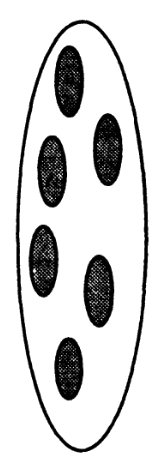
\includegraphics[height=150pt]{pictures/partons}
            \end{figure}
        \end{column}
    \end{columns}

    \footnotetext{The actual structure of the proton has a non-perturbative
    origin, so it cannot be completely understood by perturbative QFT} 
\end{frame}


\begin{frame}{LO PDF definition}
    \begin{columns}
        \begin{column}{0.55\textwidth}
            Since they are free the main property of each parton is the
            fraction of the total momentum it carries.\newline

            The probability distribution of finding a parton $p$ with momentum
            fraction $x$ it's encoded in its \textit{Parton Density Function}\footnotemark,
            $f_p(x)$.
        \end{column}
        \begin{column}{0.45\textwidth}
            Plot LO PDFs 

            %\begin{figure}
                %\centering
                %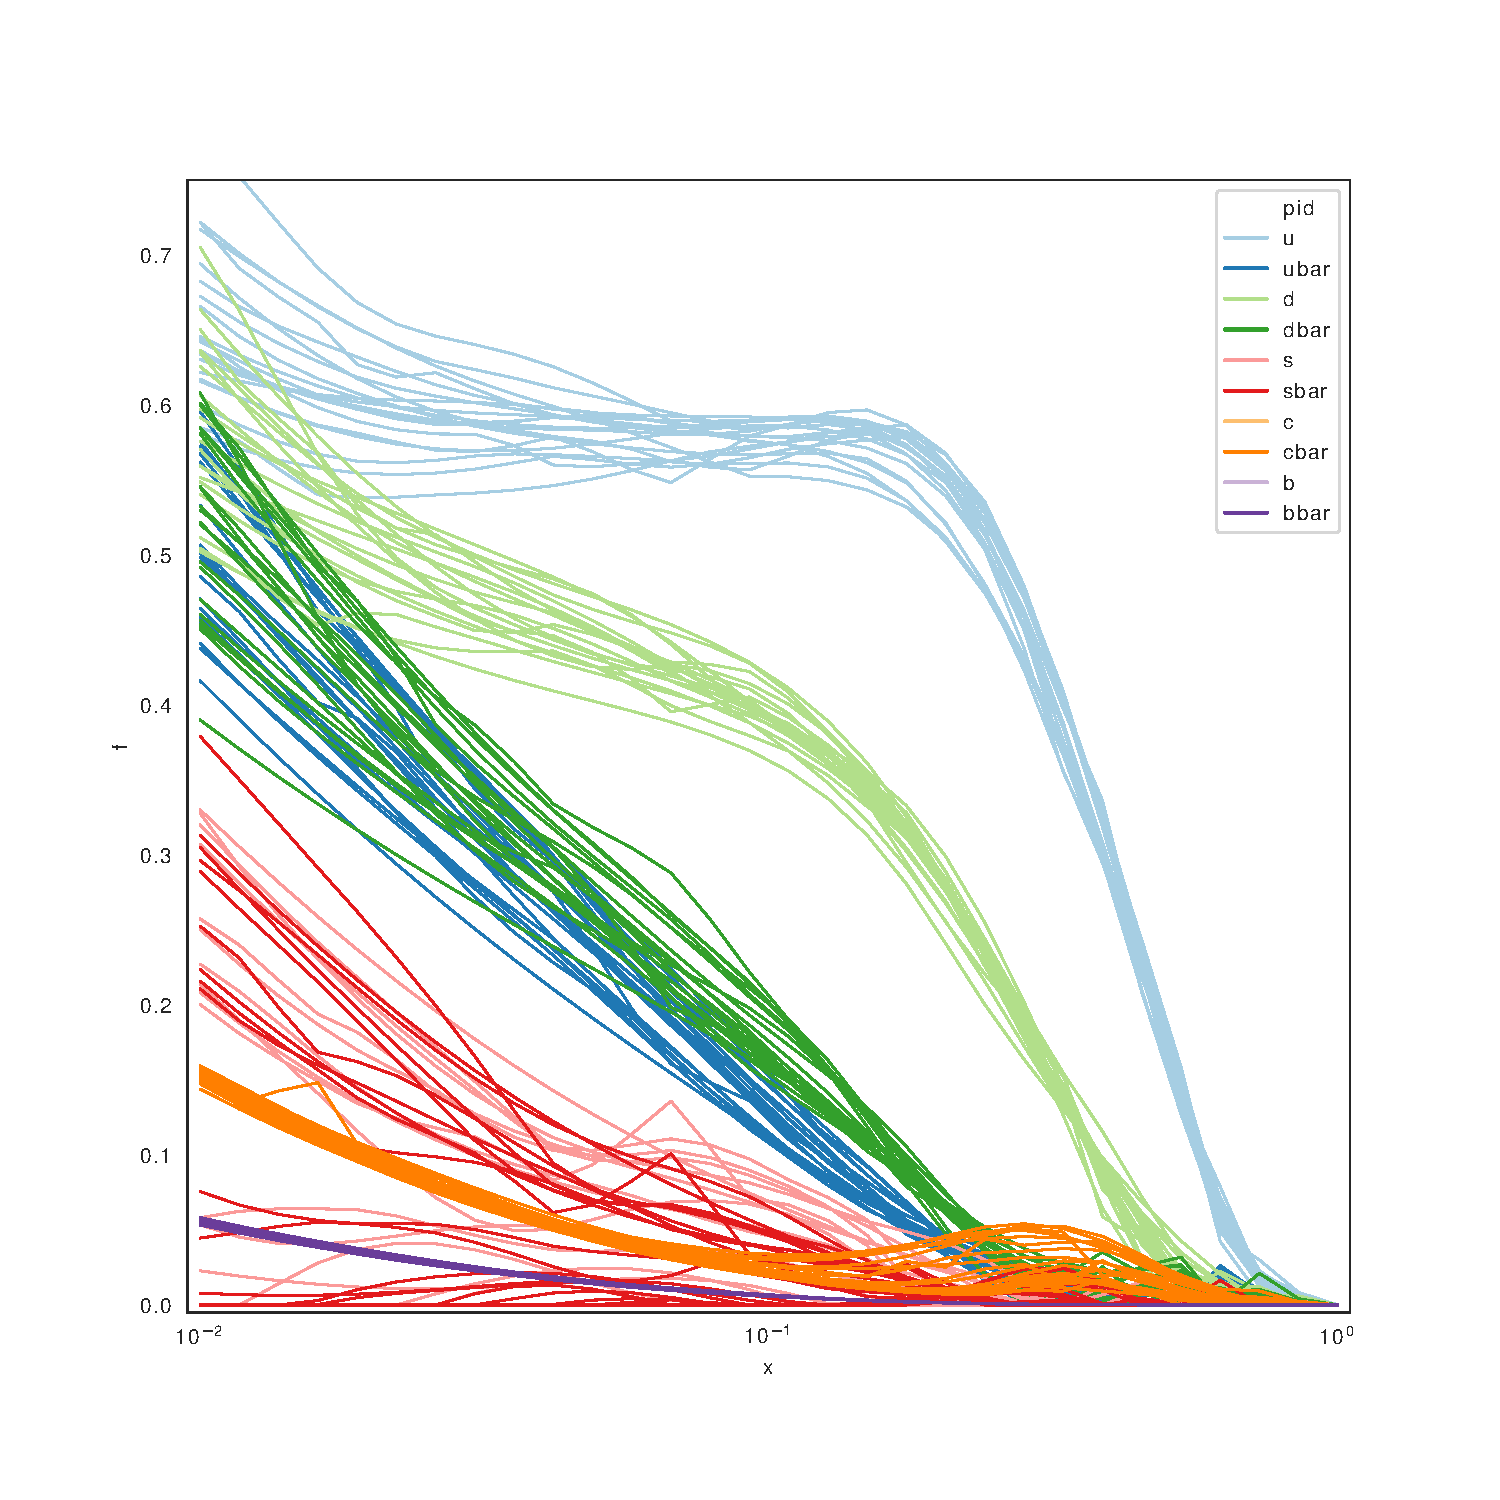
\includegraphics[height=150pt]{pictures/lo_pdfs}
            %\end{figure}
        \end{column}
    \end{columns}
    \footnotetext{In general PDFs also depend on the energy scale $Q^2$, but at
    LO they scale (see \textit{Björken scaling}). This statement can be
    explained by perturbative QCD and systematically improve, including the
    dependency through $\alpha_s$.}
\end{frame}

\section{PDF @ NLO: factorization scheme}
\begin{frame}{NLO divergences}
    As well known at NLO divergences start to appear, both in virtual and real contributions. 
    \begin{figure}
        \centering
        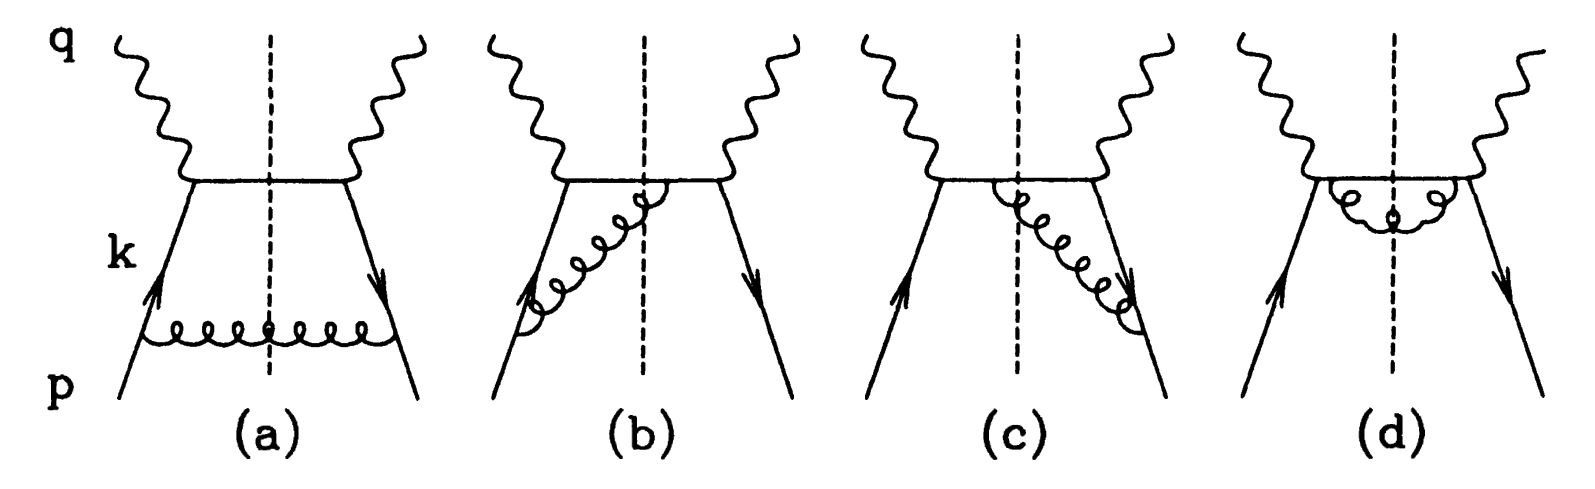
\includegraphics[width=.8\textwidth]{pictures/nlo-real}
    \end{figure}
    There are 3 kinds of divergences:
    \begin{itemize}
        \item \textbf{virtual}, due to loop integrals
        \item \textbf{soft}, due to emission of an extra soft particle
        \item \textbf{collinear}, due to 
    \end{itemize}
    The first two kind are known to cancel in sufficiently inclusive
    observables\footnote{e.g.: the KLN theorem is one of the results that guarantee
    this cancellation.}.
\end{frame}

\begin{frame}{NLO collinear divergences}
    On the other hand collinear divergences have \textit{a different origin}
    that can be related to the asymptotic freedom of strong interactions:
    
    \begin{center}
        \textit{The collinear limit corresponds to a long range (soft) part of
        the strong interaction, which is not calculable in perturbation
        theory.}
    \end{center}

    These divergences must be treated in a different way, defining a suitable
    \textbf{factorization scheme}.\newline

    Notice that collinear divergences are also responsible for the appearance
    of the characteristic $\alpha_s \log(Q^2)$, that will introduce the PDF
    dependency on $Q^2$.
\end{frame}
    
\begin{frame}{Factorization Scheme}
    The way to deal with these divergences is offered by the previous
    interpretation: we can hide them in a non-perturbative object, the PDF.
    \begin{align*}
        \hat{F}_{2,0}(x,Q^2) &= e_q^2 x \left[ \delta(1-x) +
        \frac{\alpha_s}{2\pi}\left(P(x) \log(\frac{Q^2}{\kappa^2}) +
        C(x)\right) + \dots \right]\\
        F_2(x,Q^2) &= \sum_{q,\bar{q}} q_0 \otimes \hat{F}_{2,0} (x, Q^2) =
        \sum_{q,\bar{q}} \int\limits_x^1 \frac{\dd\xi}{\xi} q_0(\xi)
        \hat{F}_{2,0}\left(\frac{x}{\xi},Q^2\right)\\
        &= \sum_{q,\bar{q}} q \otimes \hat{F}_2 (x, Q^2)\\
        q(x, \mu^2_F) &= q_0(x) + \frac{\alpha_s}{2\pi} \int\limits_x^1
        \frac{\dd \xi}{\xi} q_0(\xi) \left\{ P\left(\frac{x}{\xi}\right)
        \log(\frac{\mu^2_F}{\kappa^2}) + C\left(\frac{x}{\xi}\right)\right\} +
        \dots
    \end{align*}

    This will result in the effective \textit{subtraction} of the collinear
    divergence, the definition of a "renormalized" PDF and the appearance of a
    new unphysical energy scale: $\mu_F$, the factorization scale (which is on
    the same ground of $\mu_R$).
\end{frame}

\begin{frame}{Factorization Scheme}
    The formula for a cross section in a generic factorization scheme can be
    written as an additional counterterm contribution $\dd\sigma^C_a$, in this
    case coming from the PDF redefinition:
    \begin{align*}
        \sigma_a^{NLO}(p; \mu_F^2) &= \int\limits_{m+1} \dd\sigma^R_a(p) +
        \int\limits_{m} \dd\sigma^V_a(p) + \int\limits_{m} \dd\sigma^C_a(p;
        \mu_F^2)\\
        \dd\sigma^C_a(p;\mu_F^2) &= - \frac{\alpha_s}{2\pi}
        \frac{1}{\Gamma(1-\epsilon)} \sum_b \int\limits_0^1 \dd z \left[ -
        \frac{1}{\epsilon} \left(\frac{4\pi\mu^2}{\mu_F^2}\right)^\epsilon
        P^{ab}(z) + K^{ab}(z) \right] \dd \sigma_b^B(zp) 
    \end{align*}
    in dimensional regularization\footnote{The counterterm is such that
    $K^{ab}=0$ for $\msbar$ factorization scheme}.

    This will be useful in what follows, because it is exactly by choosing a
    specific factorization scheme (i.e. a specific $K^{ab}$ matrix) that we can
    analyze the property of the frequent $\msbar$ choice.
\end{frame}

\section{An intrinsic positive scheme}
\begin{frame}{Introduction}
    DIS scheme and similar.

    Defined on physical observables.
\end{frame}

\section{Coefficient functions NLO behaviour}
\begin{frame}{Universality of collinear structure}
    We can play this game because we know in advance that the relevant structure (the one related to the collinear subtraction) is universal.
\end{frame}

\begin{frame}{Scheme change matrix}
    How we switch scheme and $K$ properties
\end{frame}

\begin{frame}{A bunch of nontrivial positivity schemes}
    POS, MPOS, DPOS
\end{frame}

\section{Is $\msbar$ negative?}
\begin{frame}{N-space positivity $\neq$ x-space positivity}
    The easy way in \textit{N-space} and Why we need an argument in \textit{x-space}
\end{frame}

\begin{frame}{Introduction}
    Argument from MPOS -> MSbar
\end{frame}

\section{Why positivity?}
\begin{frame}{My opinion?}
    Reduce PDF variance limiting the hypothesis space. 
\end{frame}


\begin{frame}[standout]
    Thanks for your attention
\end{frame}


\end{document}
